\documentclass[10pt]{beamer}

% Beamer style
%\usetheme[secheader]{Madrid}
\usetheme{CambridgeUS}
\usecolortheme[rgb={0.65,0.15,0.25}]{structure}
%\usefonttheme[onlymath]{serif}
\beamertemplatenavigationsymbolsempty
%\AtBeginSubsection

% Packages
%\usepackage[french]{babel}
% \usepackage[latin1]{inputenc}
\usepackage{color}
\usepackage{xspace}
%\usepackage{dsfont, stmaryrd}
\usepackage{amsmath, amsfonts, amssymb}
\usepackage{url}
\usepackage{/home/robin/LATEX/Biblio/astats}
%\usepackage[all]{xy}
\usepackage{graphicx}

% Commands
\definecolor{darkred}{rgb}{0.65,0.15,0.25}
\newcommand{\emphase}[1]{\textcolor{darkred}{#1}}
%\newcommand{\emphase}[1]{{#1}}
\newcommand{\paragraph}[1]{\textcolor{darkred}{#1}}
\newcommand{\refer}[1]{{{\textcolor{blue}{{\cite{#1}}}}}}
\newcommand{\Refer}[1]{{{\textcolor{blue}{{\sl #1}}}}}
% \newcommand{\newblock}{}

% Symbols
% \newcommand{\Abf}{{\bf A}}
\newcommand{\Beta}{\text{B}}
\newcommand{\Bcal}{\mathcal{B}}
\newcommand{\BIC}{\text{BIC}\xspace}
\newcommand{\Ccal}{\mathcal{C}}
\newcommand{\dd}{\text{~d}}
% \newcommand{\dbf}{{\bf d}}
\newcommand{\Dcal}{\mathcal{D}}
\newcommand{\Esp}{\mathbb{E}}
% \newcommand{\Ebf}{{\bf E}}
\newcommand{\Ecal}{\mathcal{E}}
\newcommand{\Gcal}{\mathcal{G}}
\newcommand{\Gam}{\mathcal{G}\text{am}}
\newcommand{\Ibb}{\mathbb{I}}
% \newcommand{\Ibf}{{\bf I}}
\newcommand{\ICL}{\text{ICL}\xspace}
\newcommand{\Cov}{\mathbb{C}\text{ov}}
\newcommand{\Corr}{\mathbb{C}\text{orr}}
\newcommand{\Var}{\mathbb{V}}
\newcommand{\Vsf}{\mathsf{V}}
\newcommand{\pen}{\text{pen}}
\newcommand{\Fcal}{\mathcal{F}}
% \newcommand{\Hbf}{{\bf H}}
\newcommand{\Hcal}{\mathcal{H}}
\newcommand{\Jcal}{\mathcal{J}}
% \newcommand{\Kbf}{{\bf K}}
\newcommand{\Lcal}{\mathcal{L}}
\newcommand{\Mcal}{\mathcal{M}}
% \newcommand{\mbf}{{\bf m}}
% \newcommand{\mum}{\mu(\mbf)}
\newcommand{\Ncal}{\mathcal{N}}
% \newcommand{\Nbf}{{\bf N}}
% \newcommand{\Nm}{N(\mbf)}
\newcommand{\Ocal}{\mathcal{O}}
% \newcommand{\Obf}{{\bf 0}}
\newcommand{\Omegas}{\underset{s}{\Omega}}
% \newcommand{\Pbf}{{\bf P}}
\newcommand{\Pcal}{\mathcal{P}}
\newcommand{\Qcal}{\mathcal{Q}}
\newcommand{\Rbb}{\mathbb{R}}
\newcommand{\Rcal}{\mathcal{R}}
% \newcommand{\sbf}{{\bf s}}
% \newcommand{\Sbf}{{\bf S}}
\newcommand{\Scal}{\mathcal{S}}
\newcommand{\Ucal}{\mathcal{U}}
\newcommand{\Vcal}{\mathcal{V}}
\newcommand{\BP}{\text{BP}}
\newcommand{\EM}{\text{EM}}
\newcommand{\VEM}{\text{VEM}}
\newcommand{\VBEM}{\text{VBEM}}
\newcommand{\cst}{\text{cst}}
\newcommand{\obs}{\text{obs}}
\newcommand{\ra}{\emphase{\mathversion{bold}{$\rightarrow$}~}}
\newcommand{\QZ}{Q_{Z}}
\newcommand{\Qt}{Q_{\theta}}
%\newcommand{\transp}{\text{{\tiny $\top$}}}
\newcommand{\transp}{\text{{\tiny \mathversion{bold}{$\top$}}}}

\newcommand{\beginbackup}{
   \newcounter{framenumbervorappendix}
   \setcounter{framenumbervorappendix}{\value{framenumber}}
}
\newcommand{\backupend}{
   \addtocounter{framenumbervorappendix}{-\value{framenumber}}
   \addtocounter{framenumber}{\value{framenumbervorappendix}} 
}


% Directory
\newcommand{\figrup}{/home/robin/RECHERCHE/RUPTURES/EXPOSES/FIGURES}
\newcommand{\fignet}{/home/robin/RECHERCHE/RESEAUX/EXPOSES/FIGURES}
%\newcommand{\figmotif}{/home/robin/RECHERCHE/RESEAUX/Motifs/FIGURES}


%--------------------------------------------------------------------
\title{Two examples of Bayesian inference : exact and approximate}
  
% Bayesian model averaging of stochastic block models to estimate the graphon function 
% Averaging Stochastic Block Models to estimate the graphon function of a W-graph

\author{S. Robin}

\institute[INRA / AgroParisTech]{INRA / AgroParisTech \\
  \vspace{-.25\textheight}
  \begin{center}
  \begin{tabular}{ccccc}
    
\includegraphics[width=2.5cm]{../Figures/LogoINRA-Couleur} & 
    \hspace{.5cm} &
    
\includegraphics[width=3.75cm]{../Figures/logagroptechsolo} & 
    \hspace{.5cm} &
    
\includegraphics[width=2.5cm]{../Figures/logo-ssb}
    \\ 
  \end{tabular} 
  \end{center}
  }

\date{Laboratoire de Math�matiques de Poitiers, 29/01/2015}
%--------------------------------------------------------------------

%--------------------------------------------------------------------
%--------------------------------------------------------------------
\begin{document}
%--------------------------------------------------------------------
%--------------------------------------------------------------------

%--------------------------------------------------------------------
\frame{\titlepage}

%----------------------------------------------------------------------
\section{A reminder on Bayesian inference}
%----------------------------------------------------------------------

%----------------------------------------------------------------------
\section{Exact Bayesian inference for change-point detection}
%----------------------------------------------------------------------
%====================================================================
\frame{\frametitle{RNA-seq data} 

  $$
  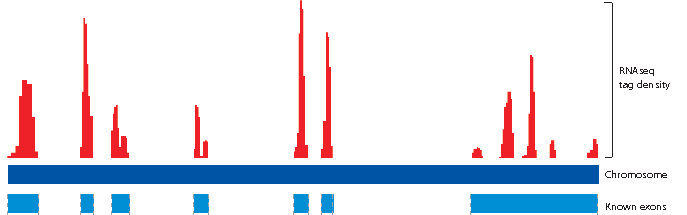
\includegraphics[width=.8\textwidth, height=.4\textheight]{\figrup/gb-2008-9-9-234-1}
  $$

  \bigskip \bigskip 
  \paragraph{New aim:} Determine if some boundaries of the transcribed regions may vary from one condition to another.
}

%====================================================================
\frame{\frametitle{Comparing transcript boundaries in yeast}

  \vspace{-.05\textheight}
  \begin{tabular}{p{.2\textwidth}p{.7\textwidth}}
    \begin{tabular}{p{.3\textwidth}}
	 One gene \\
	 \\
	 $\times$ \\
	 \\
	 Three growth \\
	 conditions: 
	 $A$, $B$, $C$
    \end{tabular}
    &
    \begin{tabular}{p{.7\textwidth}}
    \includegraphics[width=.7\textwidth]{\figrup/compyeastresult.pdf}
    \end{tabular}
  \end{tabular}
}

%====================================================================
\frame{\frametitle{Alternative transcription in yeast?}

  3 comparisons ($A/B$, $A/C$, $B/C$) $\times$ 4 change points:
  
\centerline{\includegraphics[width=.8\textwidth, height=.8\textheight]{\figrup/cred-yeast.pdf}}

}

%====================================================================
\frame{\frametitle{Bayesian 'testing'}

Define the event $E_0 =$ 'same change-point location'.

$$
\begin{array}{lccccc}
& \tau_1 & \tau_2 & \tau_3 & \tau_4 \\ 
\hline \\
P(E_0(A, B) | Y, K) & 0.32 & 0.30 &0.99 & 10^{-5} \\ \\
P(E_0(A, C) | Y, K) & 4 \; 10^{-4} & 0.99 &0.99 & 6 \; 10^{-3} \\ \\
P(E_0(B, C) | Y, K) & 5 \; 10^{-2} & 0.60 & 0.99 & 0.99 \\ \\
P(E_0(A, B, C) | Y, K) & 10^{-3} & 0.99  & 0.99 & 6 \; 10^{-3} \\ 
\end{array}
$$

\bigskip
\ra Differences at the UTR's end but not at internal exon boundaries.
}

%----------------------------------------------------------------------
\section{Approximate Bayesian inference for the stochastic block-model}
%----------------------------------------------------------------------

%--------------------------------------------------------------------
\frame{ \frametitle{{\VBEM}: Simulation study}

  \paragraph{Credibility intervals:}   $\pi_1$: $+$,
  $\gamma_{11}$: \textcolor{red}{$\triangle$}, $\gamma_{12}$:
  \textcolor{blue}{$\circ$}, $\gamma_{22}$: \textcolor{green}{$\bullet$} 
  $$
  \includegraphics[width=1\textwidth]{\fignet/im-ICQ2-2-new} 
  $$

  \pause
  \emphase{Width of the posterior credibility intervals.}
  {$\pi_1$}, \textcolor{red}{$\gamma_{11}$},
  \textcolor{blue}{$\gamma_{12}$}, \textcolor{green}{$\gamma_{22}$}
  \\
  \includegraphics[width=1\textwidth]{\fignet/im-ICQ2-3} \\

 }

%--------------------------------------------------------------------
% %--------------------------------------------------------------------
% \section{SBM analysis of biological networks}
% \frame{\frametitle{SBM analysis of biological networks}
% 
%   Joint work with J.-J. Daudin, V. Miele, F. Picard
% 
% }
% %--------------------------------------------------------------------

%-------------------------------------------------------------------- 
\frame{ \frametitle{SBM analysis of {\sl E. coli} operon networks}

  \vspace{-0.5cm}
  \hspace{-0.5cm}
  \begin{tabular}{cc}         
    \begin{tabular}{p{0.45\textwidth}}
       \onslide+<1->{
	\vspace{-1cm}
        \includegraphics[width=.45\textwidth]{\fignet/im_EcoliVEM_2} \\
          %~\\
          \refer{PMD09}
         }
    \end{tabular}
    &
    \begin{tabular}{p{0.45\textwidth}}
     \onslide+<2->{
      \vspace{-.3cm}
      \paragraph{Meta-graph representation.} \\
      %\vspace{-.5cm}
      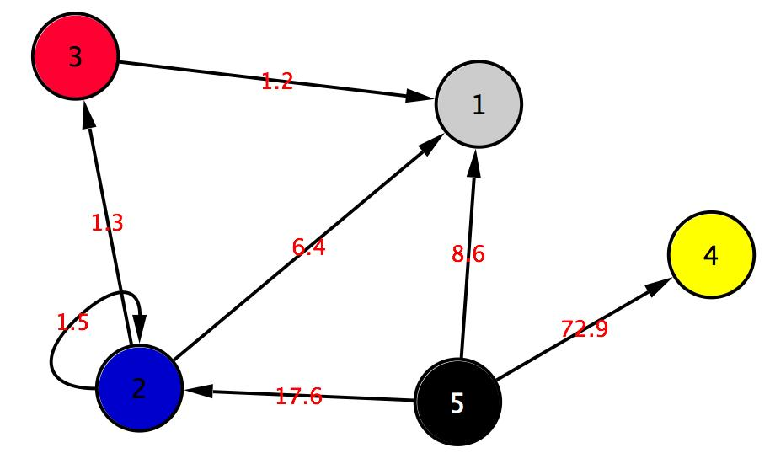
\includegraphics[width=.35\textwidth]{\fignet/VEMmetagraphe}  \\
     }
     \onslide+<3->{
      \vspace{-.3cm}
      \paragraph{Parameter estimates.} $K = 5$     \\
      \includegraphics[width=.35\textwidth]{\fignet/im-pi1BVEM}\\        
      \includegraphics[width=.35\textwidth]{\fignet/im-pi2BVEM}\\
      \includegraphics[width=.35\textwidth]{\fignet/im-pi3BVEM}\\
      \includegraphics[width=.35\textwidth]{\fignet/im-pi4BVEM}\\
      \includegraphics[width=.35\textwidth]{\fignet/im-pi5BVEM}\\
      \hline 
      \includegraphics[width=.35\textwidth]{\fignet/im-alphaBVEM}\\
     }
    \end{tabular}
  \end{tabular}
  }


%--------------------------------------------------------------------
{\tiny
  \bibliography{/home/robin/Biblio/ARC,/home/robin/Biblio/AST}%,/home/robin/Biblio/SSB}
  \bibliographystyle{/home/robin/LATEX/astats}
  %\bibliographystyle{plaine}
  }

%--------------------------------------------------------------------
\end{document}
%--------------------------------------------------------------------
%--------------------------------------------------------------------

